\section{Historia powstania fizyki kwantowej}

\subsection{Zapomnijmy o mechanice klasycznej}
Związek z nią będzie jasny, kiedy pójdziemy głębiej w teorię.

\subsection{Promieniowanie ciała doskonale czarnego}
Eksperyment Stefana-Boltzmanna (1878) badał promieniowanie cieplne emitowane przez ciało doskonale czarne.
Ciało doskonale czarne to obiekt, który pochłania całe promieniowanie i emituje je zgodnie z temperaturą.
\begin{figure}[H]
    \centering
    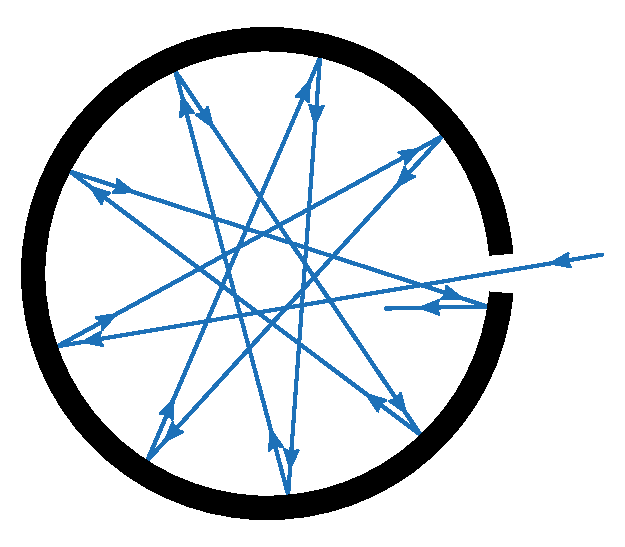
\includegraphics[width=0.3\textwidth]{blackbody}
    \caption{Ciało doskonale czarne. \textit{Źródło: Wikipedia}}
    \label{fig:blackbody}
\end{figure}

Pokazano, że całkowita energia wypromieniowywana przez takie ciało jest proporcjonalna do czwartej potęgi jego temperatury absolutnej
\begin{equation*}
    R(T) = \sigma T^4,
\end{equation*}
gdzie $R$ to moc promieniowania na jednostkę powierzchni, $T$ to temperatura w kelwinach, a $\sigma$ to stała Stefana-Boltzmanna.

Całkowita moc promieniowania to
\begin{equation*}
    R(T) = \int_0^\infty \rho(\lambda, T) d\lambda,
\end{equation*}
gdzie $\lambda$ to długość fali, a $\rho(\lambda, T)$ to spektralna funkcja rozkładu.

W 1893 Wien zauważył, że spektralna gęstość promieniowania nie zależy od $\lambda$ i $T$ osobno, ale od ich iloczynu $\lambda T$
\begin{equation*}
    \rho(\lambda, T) = \lambda^{-5} f(\lambda T).
\end{equation*}

\subsection{Prawo Rayleigha-Jeansa}
W klasycznej elektrodynamice, promieniowanie elektromagnetyczne opisane jako fale stojące daje rozkład energii w funkcji długości fali.
Liczba takich fal o długości od $\lambda$ do $\lambda + d\lambda$ to
\begin{equation*}
    \rho(\lambda, T) = \frac{8\pi}{\lambda^4} \cdot \bar{\epsilon},
\end{equation*}
gdzie $\bar{\epsilon}$ to średnia energia takiej fali.
Wzór ten jest dokładny dla długich fal, ale prowadzi do problemu z ,,katastrofą ultrafioletową'' przy krótkich falach, co zostało skorygowane przez teorię kwantową Plancka.

\begin{figure}[H]
    \centering
    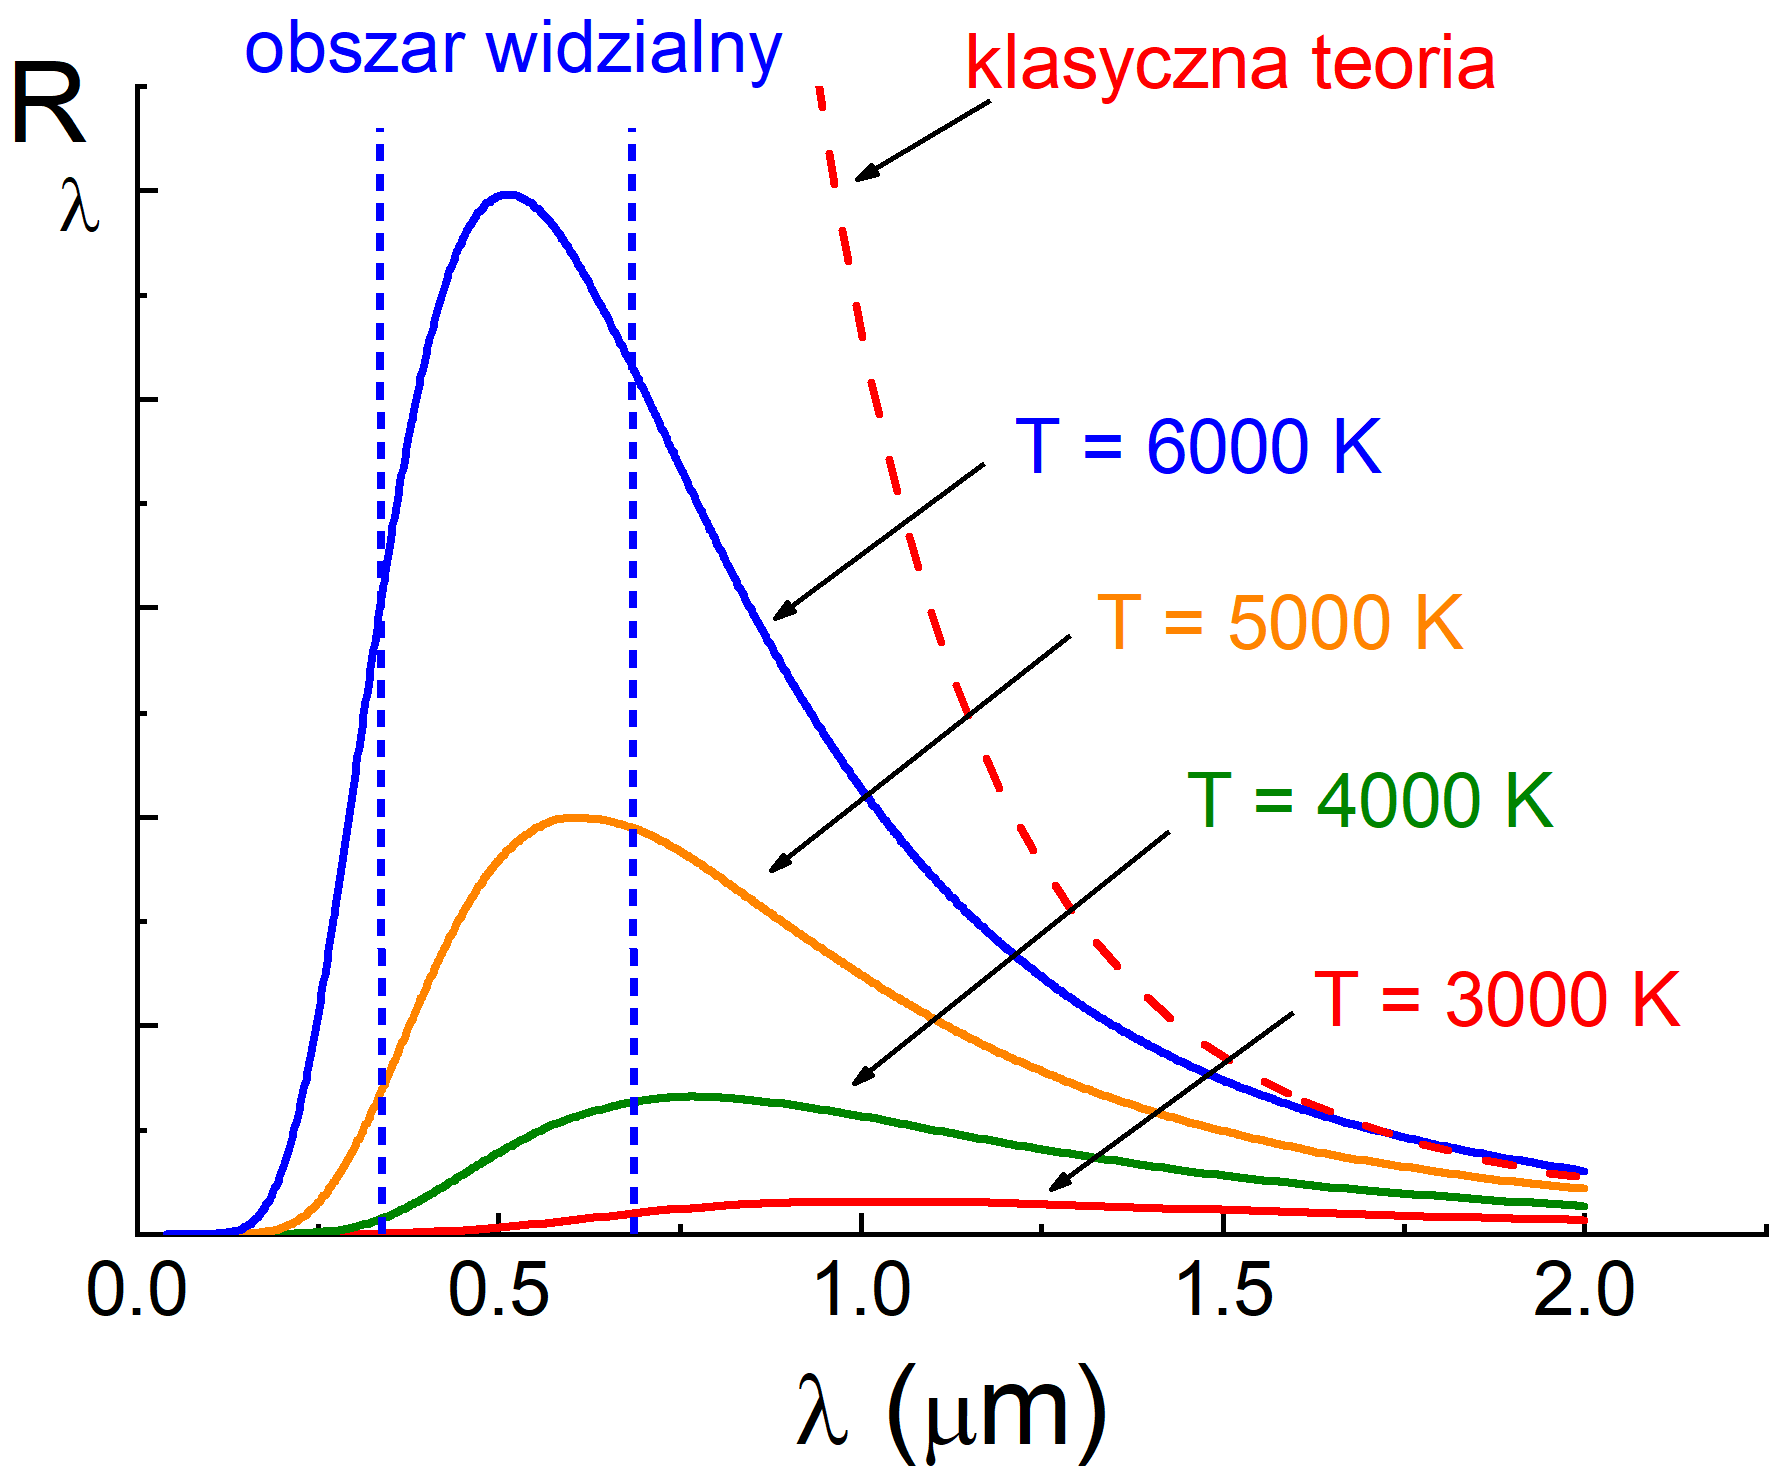
\includegraphics[width=0.5\textwidth]{widmo-promieniowania}
    \caption{Widmo promieniowania ciała doskonale czarnego w wybranych temperaturach. \textit{Źródło: Zbigniew Kąkol, Jan Żukrowski (e-Fizyka, AGH)}}
    \label{fig:widmo-promieniowania}
\end{figure}

\subsection{Teoria kwantowa Plancka}
W 1900 roku Planck zaproponował, że ciała emitują światło w postaci kwantów ($\epsilon = n\epsilon_0$)
\begin{equation*}
    \bar{\epsilon} = \frac{\sum\limits_{n=0}^{\infty} n\epsilon_0 \exp(-\frac{n\epsilon_0}{kT})}{\sum\limits_{n=0}^{\infty} \exp(-\frac{n\epsilon_0}{kT})} = \cdots = \frac{\epsilon_0}{\exp(\frac{\epsilon_0}{kT}) - 1},
\end{equation*}
gdzie \(\epsilon_0 = h \nu = \frac{h c}{\lambda}\) jest energią jednego kwantu promieniowania.

Z tego wyrażenia Planck otrzymał rozkład promieniowania w funkcji długości fali, który ma postać
\begin{equation*}
    \beta(\lambda, T) = \frac{8\pi hc}{\lambda^5} \cdot \frac{1}{\exp(\frac{hc}{k\lambda T}) - 1},
\end{equation*}
Wzór ten zgadza się z wynikami eksperymentalnymi, eliminując problem ,,katastrofy ultrafioletowej''.

\subsection{Efekt fotoelektryczny}
Efekt fotoelektryczny to zjawisko emisji elektronów z powierzchni metalu pod wpływem padającego na niego światła.

\begin{figure}[H]
    \centering
    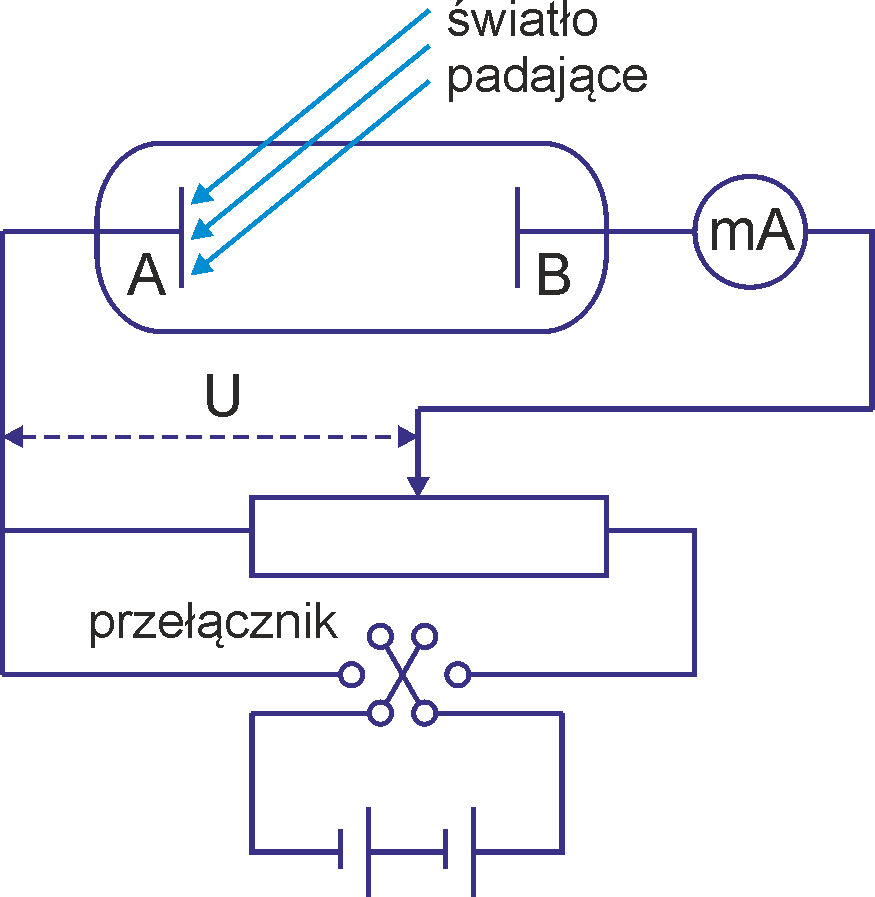
\includegraphics[width=0.5\textwidth]{efekt-fotoelektryczny}
    \caption{Układ do obserwacji zjawiska fotoelektrycznego. \textit{Źródło: Zbigniew Kąkol, Jan Żukrowski (e-Fizyka, AGH)}}
    \label{fig:efekt-fotoelektryczny}
\end{figure}

W 1900 roku doświadczenia Lenarda wykazały, że energia elektronów zależy od częstotliwości światła, a nie jego intensywności.
Einstein sformułował wzór efektu fotoelektrycznego
\begin{equation*}
    \frac{1}{2} m v_{\max}^2 = h\nu - W,
\end{equation*}
gdzie $W$ to funkcja pracy metalu (zależna od rodzaju metalu).

\subsection{Widma atomowe i model Bohra}
Newton (1660) badał rozszczepienie światła. Melvill (1755) odkrył, że różne pierwiastki mają charakterystyczne linie widmowe. Kirchhoff (1855) zauważył, że widmo zależy od typu atomu i istnieją zarówno widma emisyjne, jak i absorpcyjne.

Balmer (1885) podał wzór:
\begin{equation*}
    \lambda = C \cdot \frac{n^2}{n^2 - 4}.
\end{equation*}

Rydberg sformułował bardziej ogólny wzór:
\begin{equation*}
    \tilde{\nu} = R_H \left( \frac{1}{2^2} - \frac{1}{n^2} \right).
\end{equation*}
